\documentclass[10pt,pdf,hyperref={unicode}]{beamer}% тип документа
% далее идёт преамбула
\usepackage{tikz}
\usetikzlibrary{graphs}
\usepackage[T1,T2A]{fontenc}
\usepackage[utf8]{inputenc}
\usepackage[english,russian]{babel}
%\usepackage{amsmath}
%\usepackage{amsfonts}
%\usepackage{amssymb}
%\usepackage{makeidx}

\usepackage[english,russian]{babel}
\usetheme{Berlin}

\title{Информационные процессы и технологии}
\author{Романцов Григорий Дмитриевич}
\date{}
\begin{document}% начало презентации

\begin{frame}% первый слайд
  \titlepage
\end{frame}

\begin{frame}{Информационные технологии}

\textbf{Информационные технологии} - это процессы, методы поиска, сбора, хранения, обработки, предоставления, распространения информации и способы осуществления таких процессов и методов.

\end{frame}

\begin{frame}{Информационные технологии}
  % \includegraphics[width=\textwidth]{cs_map.png}
  Информационные технологии могут быть сгруппированы следующим образом:
  \begin{itemize}
    \item технические средства
    \item коммуникационные средства
    \item организационно-методическое обеспечение
    \item стандартизация
  \end{itemize}
\end{frame}

\begin{frame}{Информационные процессы}
  \begin{itemize}
    \item{\textbf{ЭВМ}} --- это комплекс технических, аппаратных и программных средств, предназначенных для автоматической обработки информации, вычислений, автоматического управления.
    \item Объект передачи и преобразования в вычислительных системах --- \textit{информация}
  \end{itemize}
\end{frame}

\begin{frame}{Информационные процессы}
  \textbf{Информатика} состоит из трех составных частей:
  \begin{itemize}
    \item теории передачи и преобразования информации;
    \item алгоритмических средств обработки информации;
    \item вычислительных средств;
  \end{itemize}
\end{frame}

\begin{frame}{Информационные процессы}
\begin{minipage}{0.4\textwidth}
  \begin{itemize}
\item сбор данных
\item формализация данных
\item фильтрация данных
\item сортировка данных
\item группировка данных
\end{itemize}
\end{minipage}
\hfill
\begin{minipage}{0.4\textwidth}
  \begin{itemize}
\item архивация данных
\item защита данных
\item транспортировка данных
\item преобразование данных
\end{itemize}
\end{minipage}
\end{frame}

\begin{frame}{Позиционные системы счисления}
  $$x = \sum^{n-1}_{k=0} a_{k}b^{k}$$
  \begin{itemize}
    \item где, $a_{k}$ --- это целые числа, называемые цифрами, удовлетворяющие неравенству $0 \leq  a_{k} \leq b - 1$
    \item каждая степень $b^{k}$ в такой записи называется весовым коофицентом разряда
    \item старшенство разрядов определяется значением показателя $k$ (номером разряда)
  \end{itemize}
\end{frame}

\begin{frame}{Перевод из десятичной в двоичную}
  \begin{figure}[h]
    \center{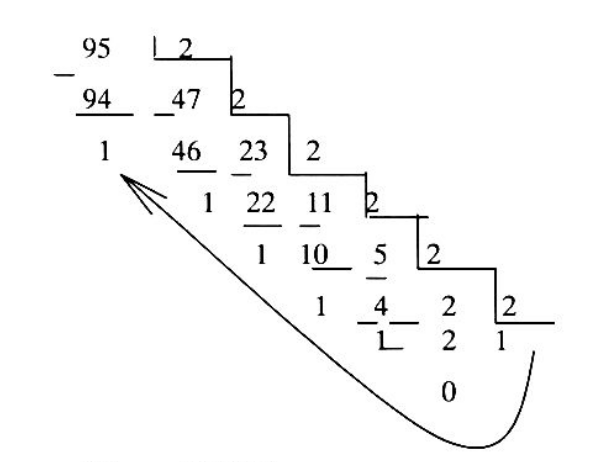
\includegraphics[width=128pt]{dectobin.png}
      \label{ris:dectooct}}
  \end{figure}
\end{frame}


\begin{frame}{Перевод из десятичной в восьмеричную}
  \begin{figure}[h]
    \center{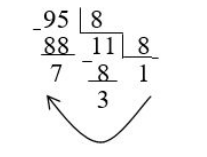
\includegraphics[width=128pt]{dectooct.png}
      \label{ris:dectooct}}
  \end{figure}
\end{frame}

\begin{frame}{Перевод из десятичной в шестьнадцатеричную}
  \begin{figure}[h]
    \center{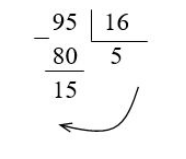
\includegraphics[width=128pt]{dectohex.png}
      \label{ris:dectooct}}
  \end{figure}
\end{frame}


\begin{frame}
  \begin{table}[h]
  \caption{Соответствие цифр в разных системах счисления}
  \begin{center}\label{tab:octhex}
    \begin{tabular}{|c|c|c|}
      \hline
     Символы & k - 3 & k - 4 \\
     \hline
      0 & 000 & 0000 \\
      1 & 001 & 0001 \\
      2 & 010 & 0010 \\
      3 & 011 & 0011 \\
      4 & 100 & 0100 \\
      5 & 101 & 0101 \\
      6 & 110 & 0110 \\
      7 & 111 & 0111 \\
      8 &     & 1000 \\
      9 &     & 1001 \\
      A &     & 1010 \\
      B &     & 1011 \\
      C &     & 1100 \\
      D &     & 1101 \\
      E &     & 1110 \\
      F &     & 1111 \\
      \hline
     \end{tabular}
  \end{center}
\end{table}

\end{frame}

\begin{frame}{Цифровое представление данных}
  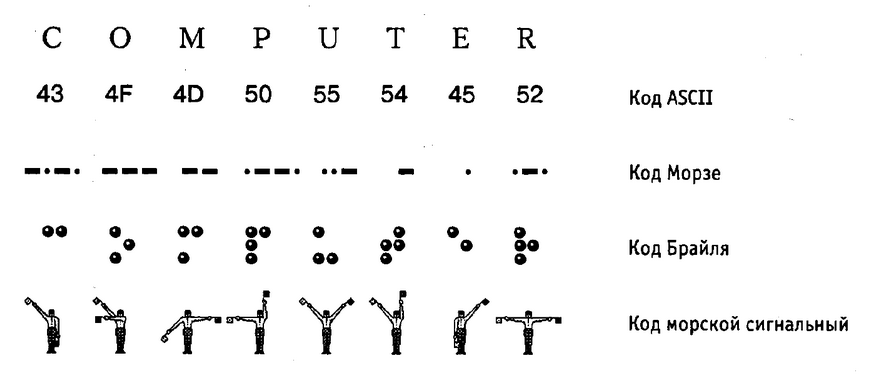
\includegraphics[width=\textwidth]{p1.png}
\end{frame}


\begin{frame}{Цифровое представление данных}
  $$0\;1$$
  $$00\; 01\; 10\; 11$$
  $$000\; 001\; 01\; 011\; 100\; 101\; 110\; 111$$
    $$N=2^{m}$$
  где:

  N --- количество независимых кодируемых значений;
  m --- разрядность двоичного кодирования, принятая в данной системе;

\end{frame}

\begin{frame}{Цифровое представление данных}

$$19:2 = 9+1$$
$$9 : 2 = 4 + 1$$
$$4 : 2 = 2 + 0$$
$$2:2 = 1$$
\center{Таким образом: $19_{10} = 1011_{2}$}
\end{frame}

\begin{frame}{Кодирование текстовых данных}
   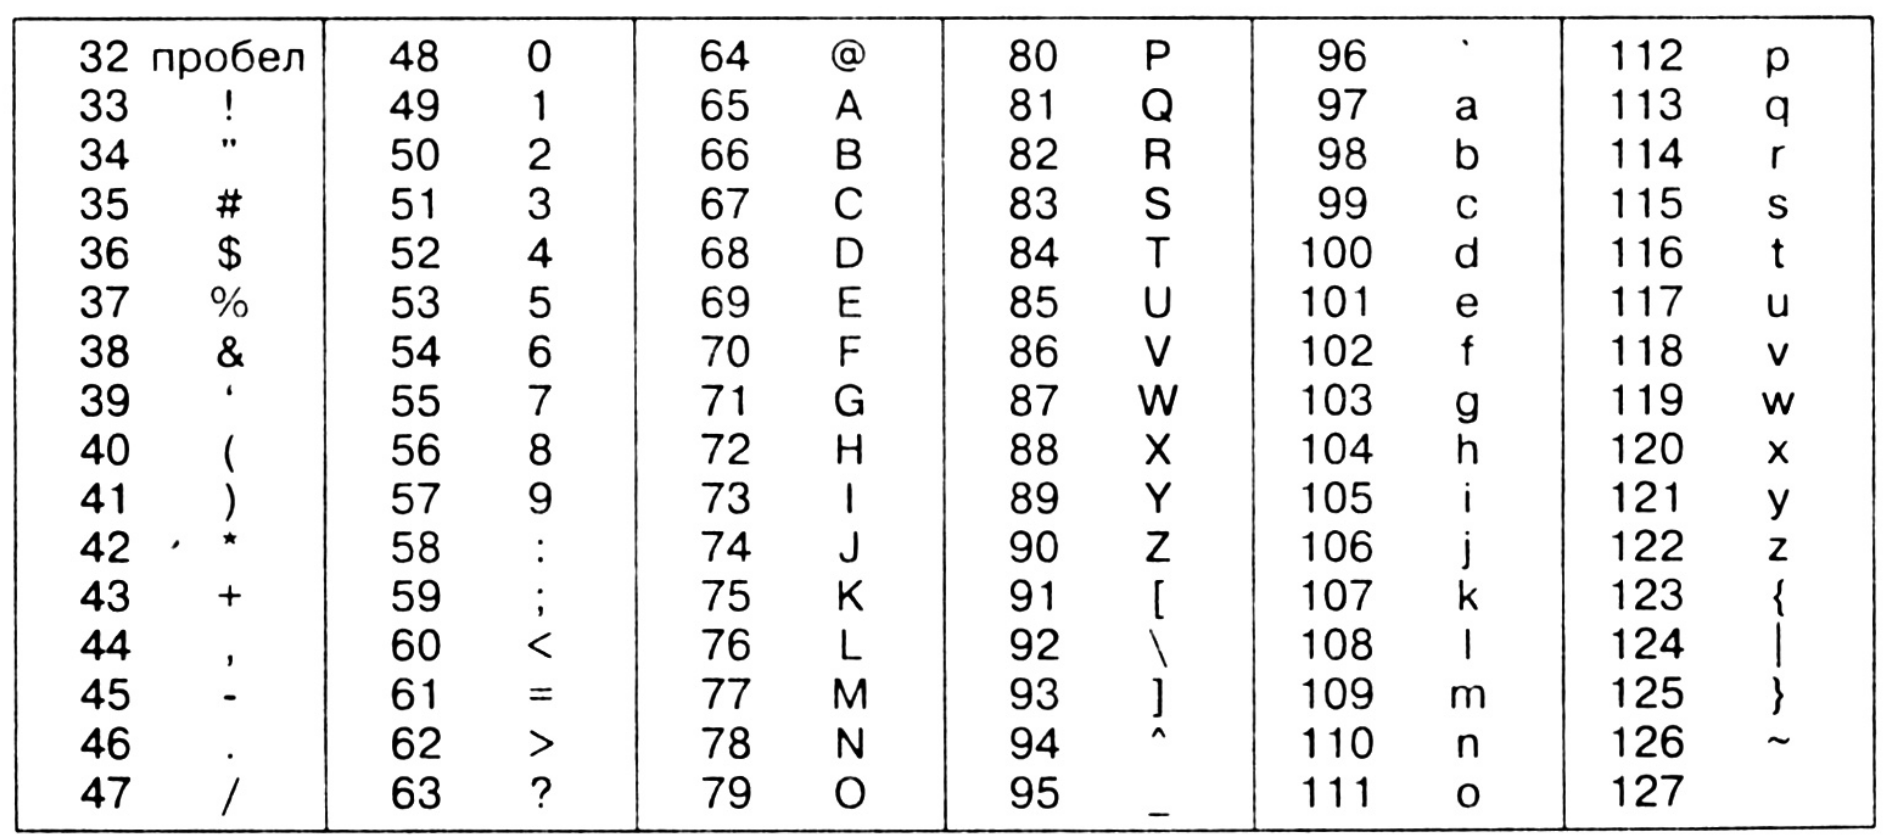
\includegraphics[width=\textwidth]{p2.png}
\end{frame}

\begin{frame}{Кодирование изображений}
  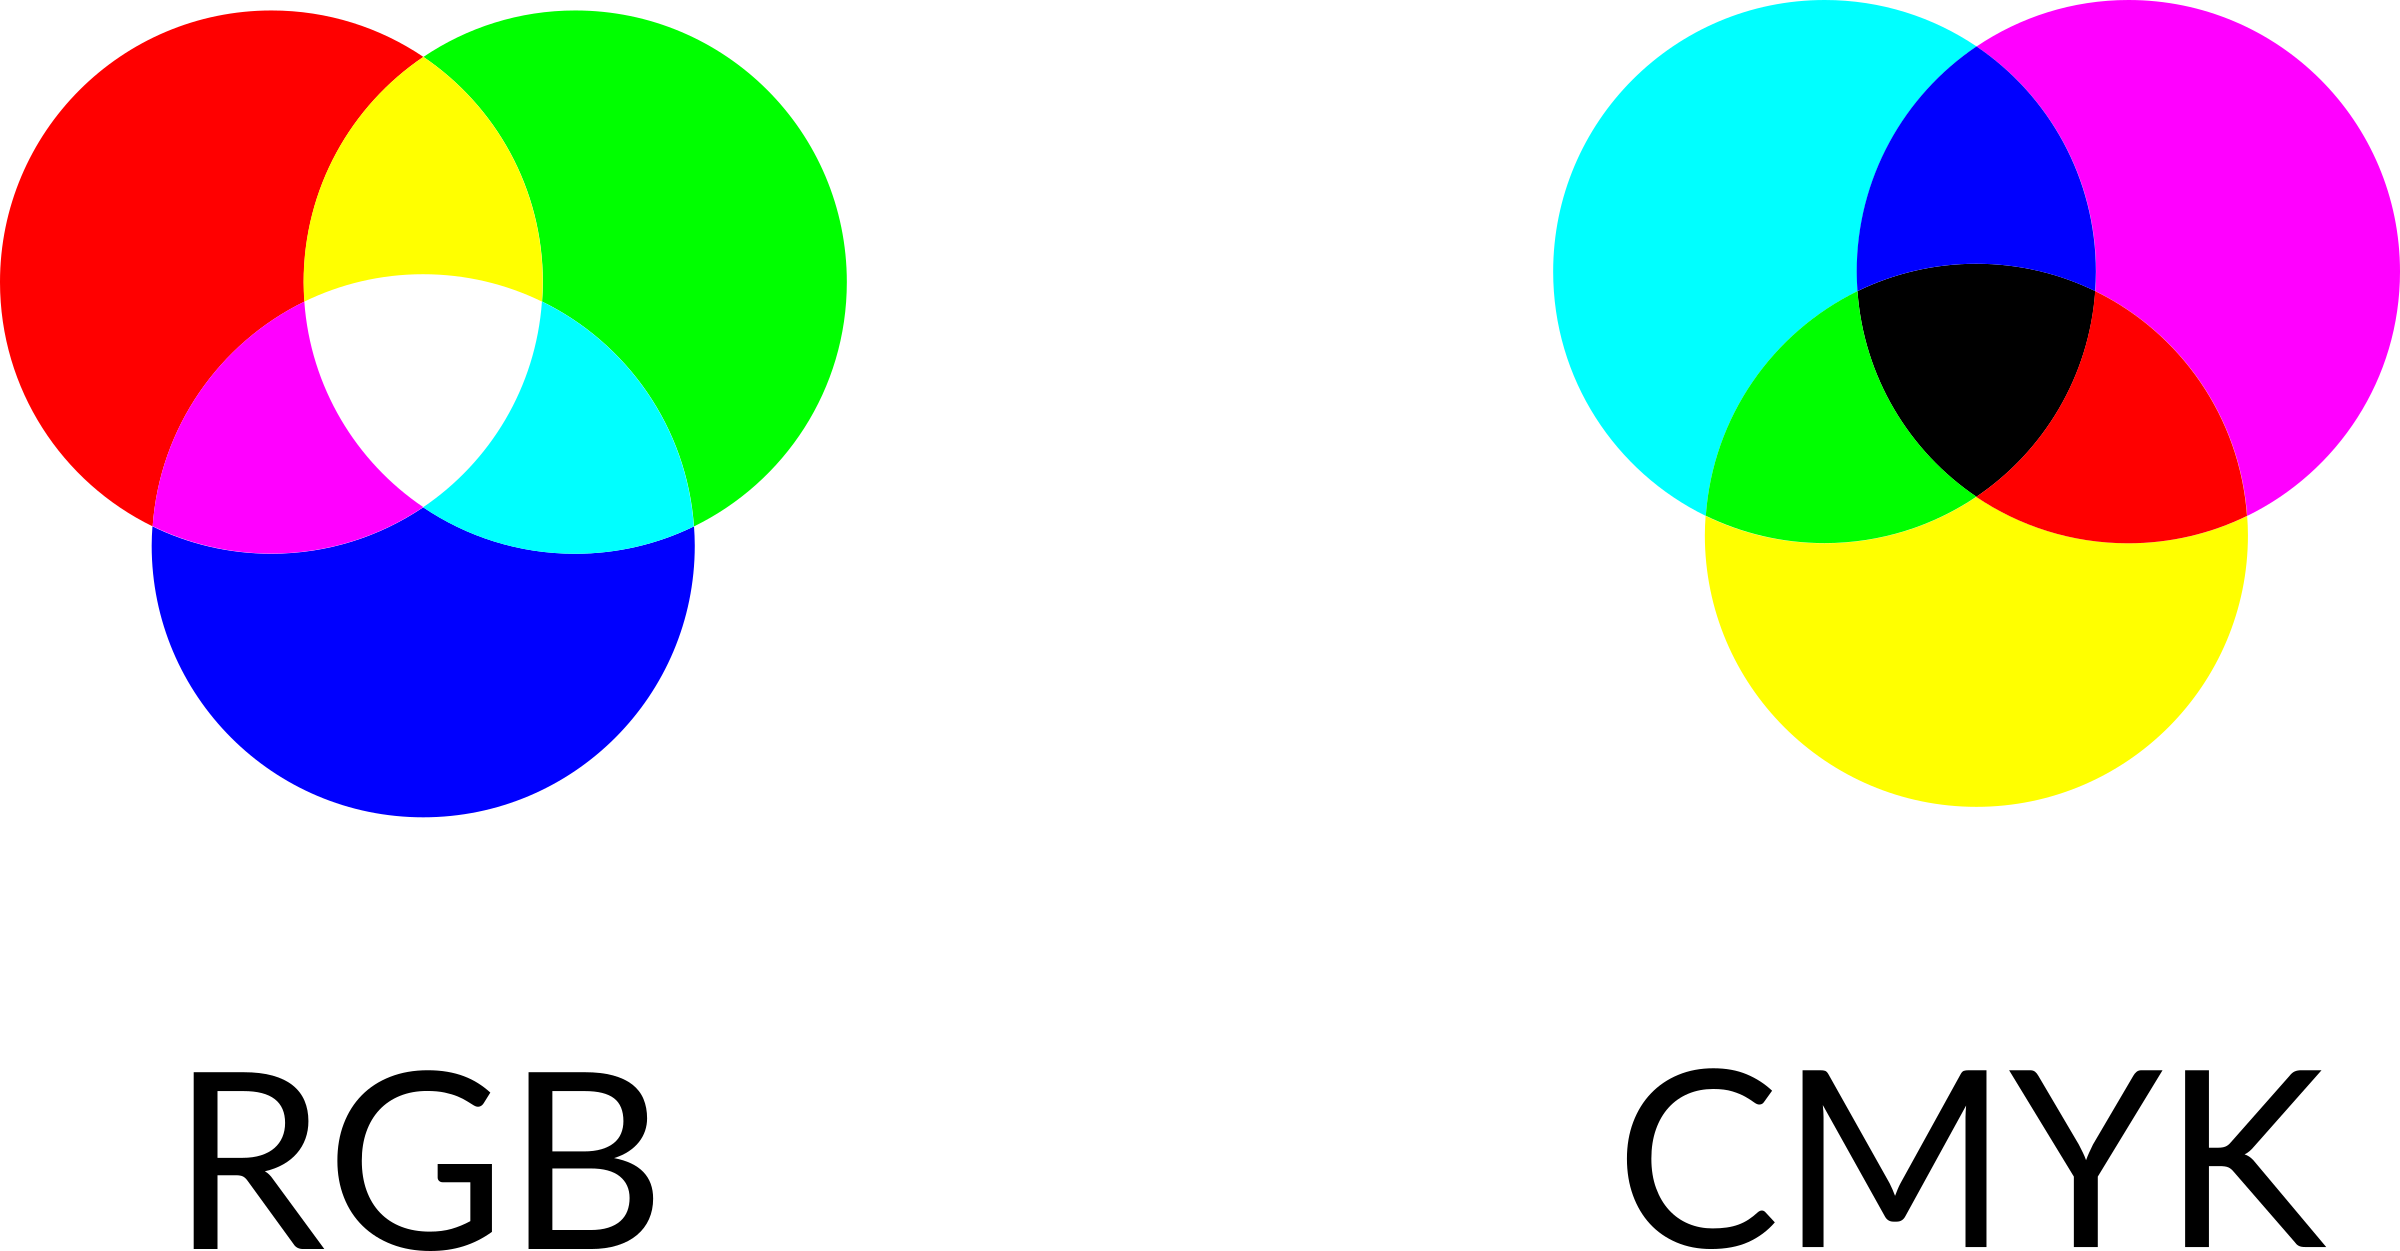
\includegraphics[width=\textwidth]{p3.png}
\end{frame}

\begin{frame}{Кодирование звуков}
  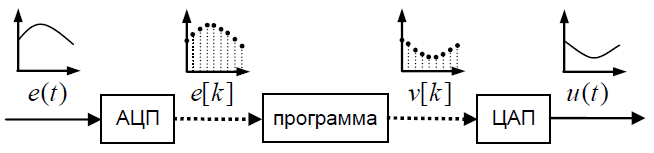
\includegraphics[width=\textwidth]{p4.png}
\end{frame}

\begin{frame}{Еденицы измерения данных}
  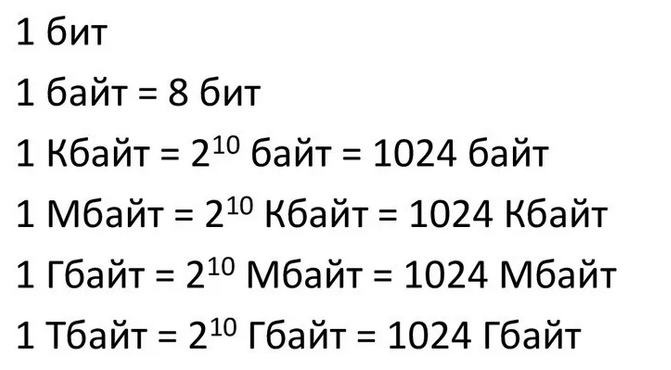
\includegraphics[width=\textwidth]{p5.png}
\end{frame}

\begin{frame}{Еденицы хранения данных}
  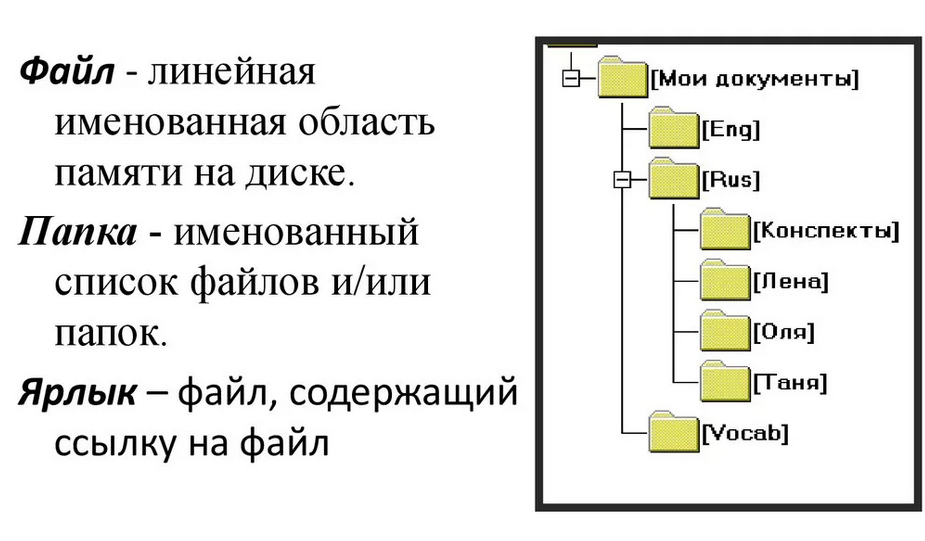
\includegraphics[width=\textwidth]{file.png}
\end{frame}

\begin{frame}{Носители информации}
  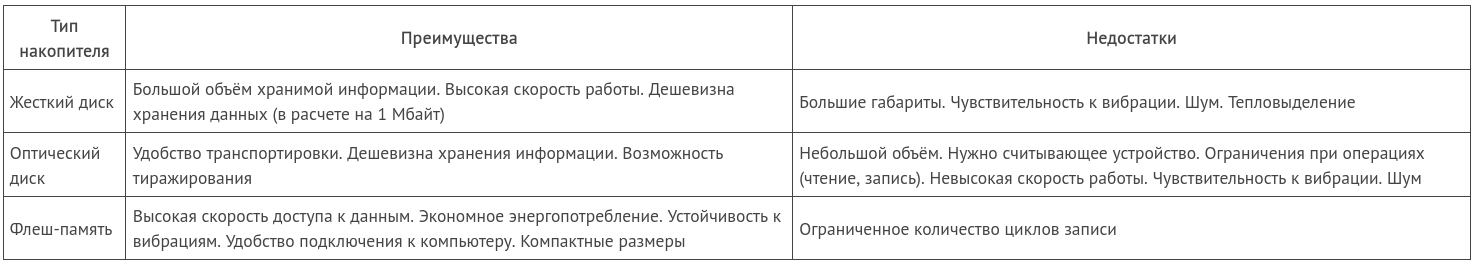
\includegraphics[width=\textwidth]{p6.png}
\end{frame}

\begin{frame}{Базовая конфигурация компьютера}
  \begin{minipage}{0.4\textwidth}
  \begin{itemize}
    \item системный блок;
    \item монитор;
    \item клавиатура;
    \item мышь;
\end{itemize}
\end{minipage}
\hfill
  \begin{minipage}{0.4\textwidth}
          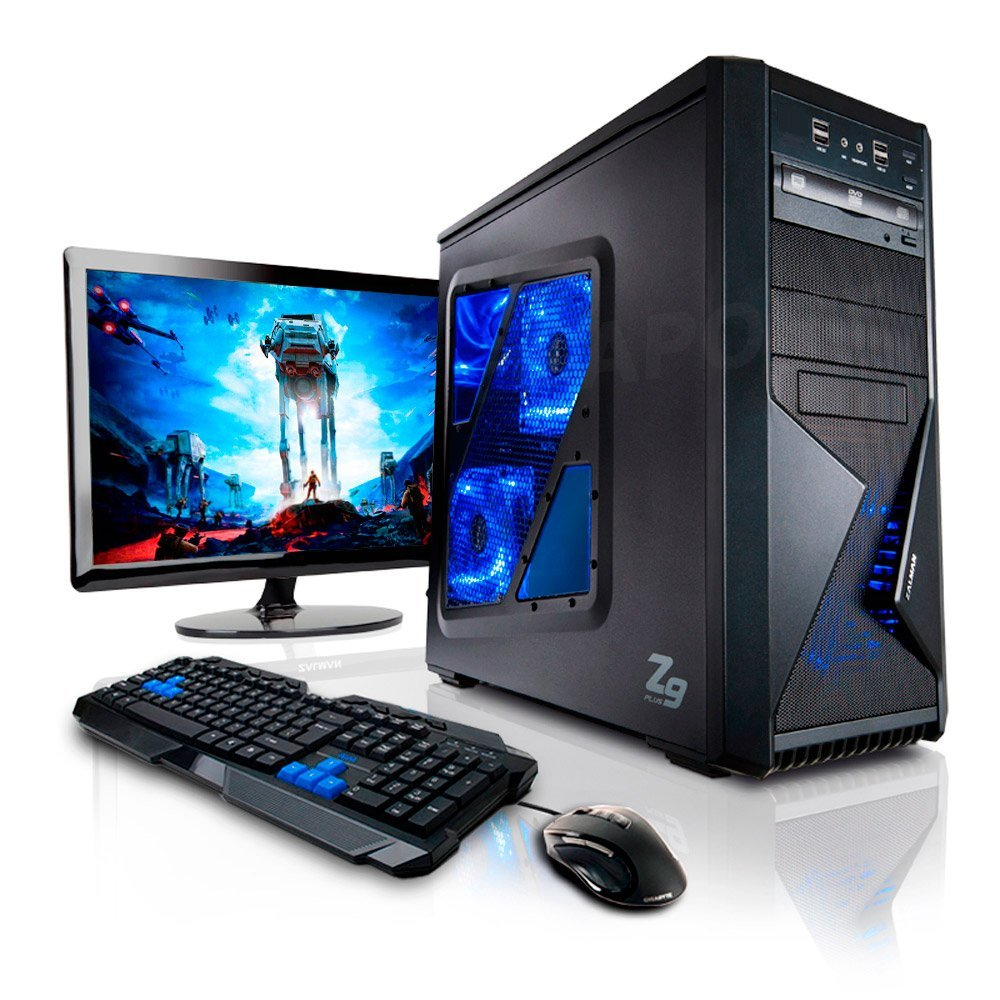
\includegraphics[width=\textwidth]{p7.png}
  \end{minipage}
\end{frame}

\begin{frame}{Внутреннее устройство компьютера}
  \begin{minipage}{0.4\textwidth}
    \begin{itemize}
    \item материнская плата;
    \item процессор;
    \item чипсет;
    \item шины;
    \item оперативная память;
    \item пзу;
    \item видеокарта;
    \end{itemize}
\end{minipage}
\hfill
  \begin{minipage}{0.4\textwidth}
          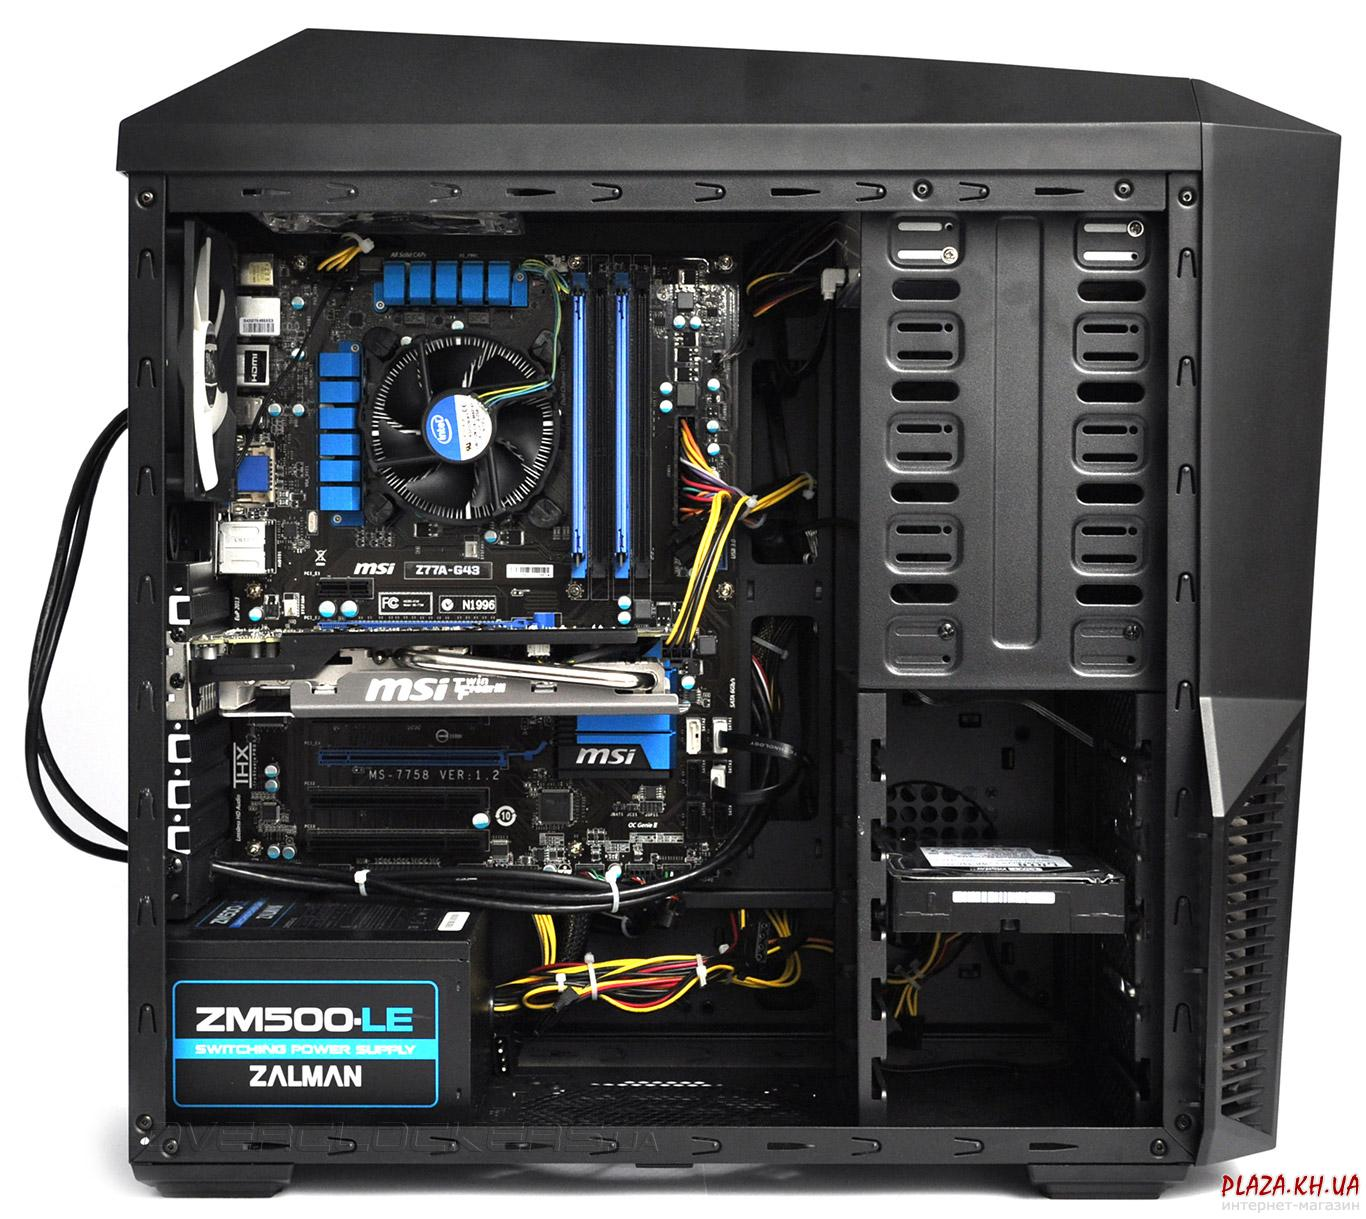
\includegraphics[width=\textwidth]{p8.png}
  \end{minipage}
\end{frame}

\begin{frame}{Носители информации}
  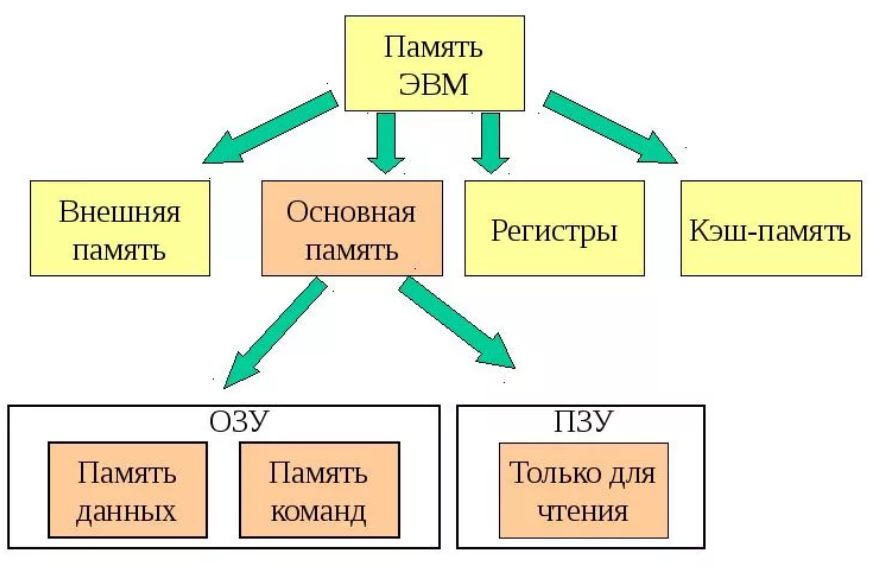
\includegraphics[width=\textwidth]{mem_l.png}
\end{frame}

\begin{frame}{Хранение информации на ЭВМ}
  \begin{minipage}{0.4\textwidth}
    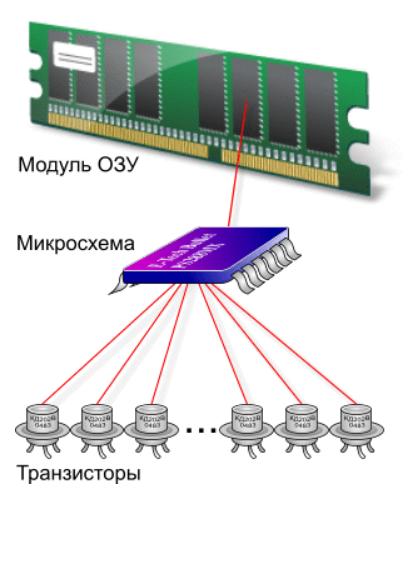
\includegraphics[width=\textwidth]{ozu.png}
\end{minipage}
\hfill
  \begin{minipage}{0.4\textwidth}
    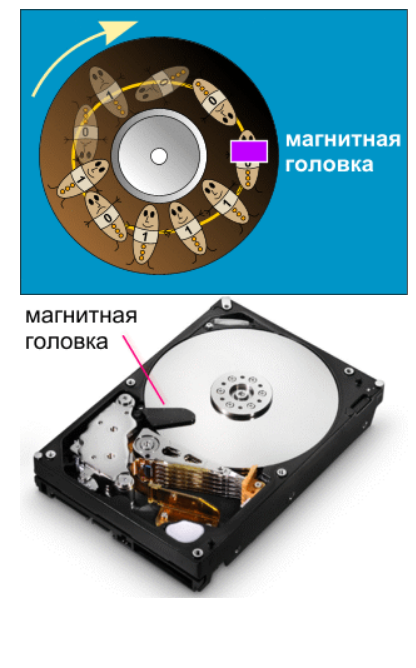
\includegraphics[width=\textwidth]{pzu.png}
  \end{minipage}
\end{frame}

\begin{frame}{Сжатие данных}
  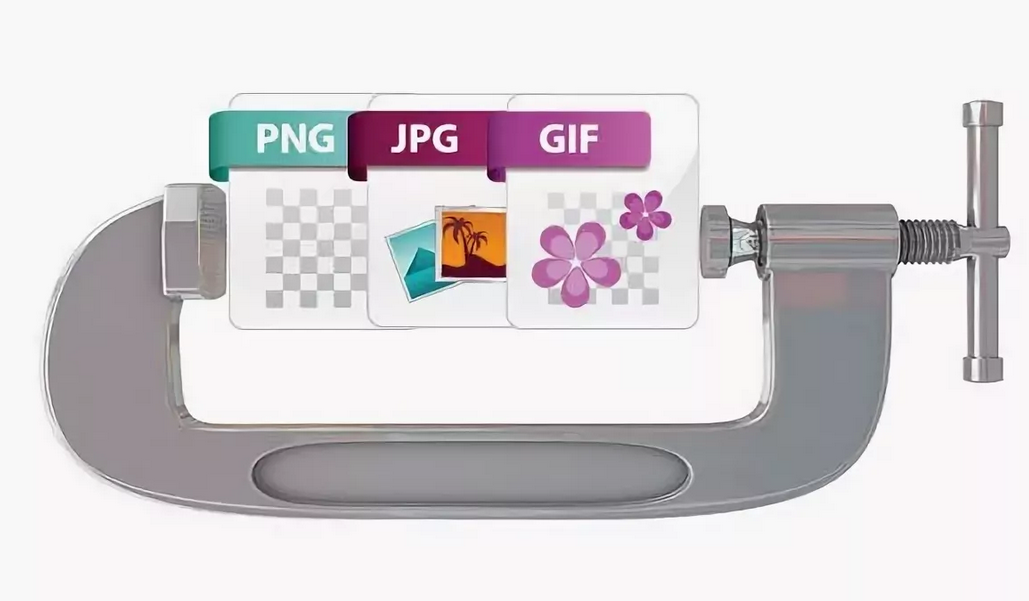
\includegraphics[width=\textwidth]{zip.png}
\end{frame}

\begin{frame}{Язык запросов поисковиков}
  
\includegraphics[width=\textwidth]{search.png}
\end{frame}

\end{document}
